%TEX root = ../dissertation.tex

\chapter{Implementation}
\label{chapter:implementation}
To demonstrate the architecture feasibility and validity, a proof of concept implementation has been developed by means of extending an existing \gls{SDN} controller.
The requirements set for the choice of the controller were controller completeness, popularity and availability of source code, which lead to a final decision between OpenDaylight\cite{OpenDaylight} and Floodlight\cite{Floodlight}\cite{Kreutz2014}\cite{ControllerComparison}.\\
%
%Justify choice of Floodlight
While both OpenDaylight and Floodlight are modular open-source \gls{SDN} controllers implemented in Java, highly popular and supported by major players in the networking industry\cite{OpenDaylight}\cite{Floodlight}, however, at the time of the decision, Floodlight, which was at version 1.1, had a more stable implementation when compared with the OpenDaylight, which was at release Helium.
OpenDaylight also offers support for multiple Southbound Interface protocols, which while falling outside the scope of this work renders the platforms architecture more complex than that of Floodlight, and would therefore add more complexity to the implementation.
For these reasons, Floodlight was chosen as a basis for the implementation of proof of concept for the proposed architecture.\\
%
\section{Elastic SDN controller cluster}
\label{section:SDN-controller-cluster-implementation}
% Floodlight
Floodlight is a modular implementation of a \gls{SDN} controller developed by Big Switch Networks using the Java language, and is currently in version 1.1.
Floodlight shares its core implementation with Big Switch Networks's own Big Network Controller\cite{Floodlight}.
It offers stable support for OpenFlow versions 1.0 and 1.3 and experimental support for versions 1.1, 1.2 and 1.4 through OpenFlowJ Loxi, a library that encapsulates the OpenFlow protocol and exposes functionality through a protocol version agnostic \gls{API}\cite{LoxiGen}.\\
Floodlight's architecture is highly modular, composed by a base \emph{Module Loading System} that loads a set of registered modules, allowing for the establishment of inter-module dependencies as well as service exposure and consumption by registered modules\cite{FLArch}.
There are a set of \emph{Controller Modules} which implement core \gls{SDN} controller functionality which is then either exposed by service \glspl{API} or by propagating as events to registered listener modules, thus enabling an event-driven programming model.
These modules implement features such as OpenFlow switch management connection handling (FloodlightProvider and OFSwitchManager modules), inter-switch link discovery through \gls{LLDP} and \gls{BDDP} (LinkDiscoveryManager module), network host discovery and tracking through packet-in inspection (DeviceManagerImpl module) and network topology and routing service (TopologyService module).\\
Floodlight defines a unique device as a (\gls{VLAN};\gls{MACAddress}) pair and considers that there may be at most one attachment point per network domain \cite{FLArch}.
In order to maintain compatibility the same concepts were taken into consideration for the implementation of the proof of concept.\\
%NOTE: DeviceManagerImpl "By default the entity classifier uses MAC address and VLAN to identify a device. These two properties will define what is unique as a device. (...) A device can have as many as one attachment point per OpenFlow island, where an island is defined as a strongly connected set of OpenFlow switches talking to the same Floodlight controller."
%
\subsection{Proof of concept implementation}
\label{subsection:poc-module}
%
% Highlevel description
The proof of concept implementation followed Floodlight's architectural design.
A floodlight module was therefor implemented, encapsulating all the clustering concepts stated in chapter \ref*{chapter:architecture} section \ref{section:SDN-controller-cluster} and both providing \glspl{API} and triggering events to registered listeners.
The main building blocks composing the developed module depicted in figure \ref{fig:amorphous_block_diagram} are as follows:
%
\begin{figure}
	\centering
	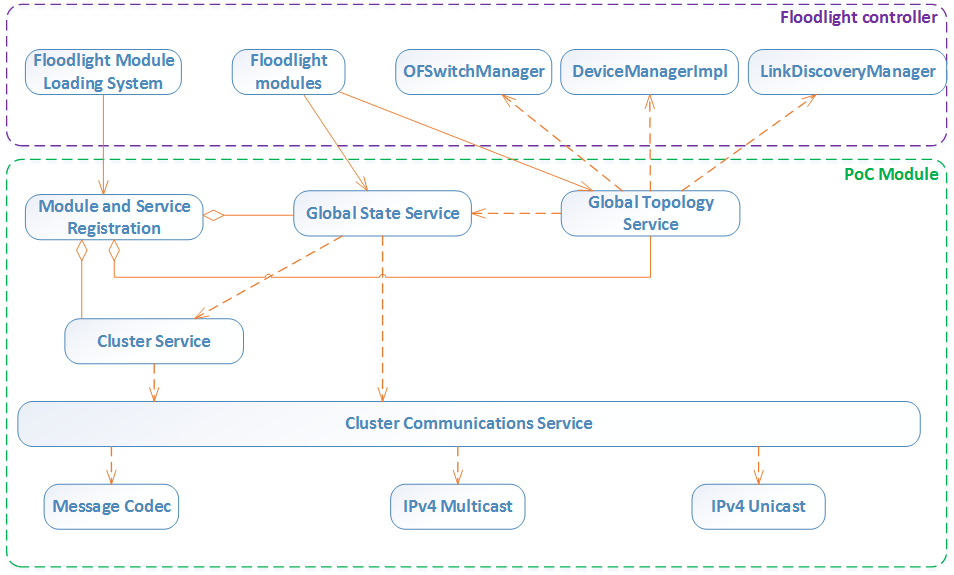
\includegraphics[scale=0.65]{amorphous_block_diagram}
	\caption{Proof of concept implementation high level block diagram}
	\label{fig:amorphous_block_diagram}
\end{figure}
%
\begin{itemize}
	\item \textbf{Module and Service registration:} Handles all the tasks necessary to integrate with the Floodlight controller, including component initialization, declaring dependencies and exposing the services provided by both Global State Service and Global Topology Service by implementing the IFloodlightModule interface, which is then used by the Floodlight Module Loading System to register and execute the module.
	%
	\item \textbf{Global State Service:} Handles the global state of the \gls{MIB} and exposes an \gls{API} to provide message exchange between Floodlight modules executed in different instances of the cluster, therefore allowing for the extension and enhancement of the distributed environment properties to module specific implementations. The message exchange \gls{API} provided is based on the concept of message queues, in which a module registers in a queue and is allowed to send messages to and listen for incoming messages on the queue. This module depends on the Cluster Communications Service to exchange messages with peer controller instances and on the Cluster Service in order to determine the address of the destination peer and whether or not a peer is a member of the cluster.
	%
	\item \textbf{Global Topology Service:} Locally, it provides the same services as the TopologyService module by exposing an \gls{API} to be consumed by other Floodlight modules and triggering events upon topology changes, using however the Global State Service's \gls{MIB} instead of the local \gls{MIB}. It also listens for local topology changes, such as new OpenFlow switch connections, new inter-switch links and hosts, updating its \gls{MIB} and propagating the changes to peer instances accordingly. This block registers to a special queue in Global State Service reserved for the exchange of the messages specified in table \ref{table:cluster-message-spec} under the scope of gls{MIB} update. All messages queued for sending through the exposed \gls{API} are sent encapsulated (and de-encapsulated when received before being registered to the corresponding queue) within a special purpose container message that holds properties such as the queue identifier.
	%
	\item \textbf{Cluster Service:} This block is responsible for all the clustering logic such as that of the registration of peer cluster instances (including the registration of the local instance with existing ones) described in chapter \ref*{chapter:architecture} section \ref{section:SDN-controller-cluster} and the exchanging and processing of all the messages stated in table \ref{table:cluster-message-spec} under the scope of cluster membership. Messages are sent and received using the \gls{API} provided by the Cluster Communications Service.
	%
	\item \textbf{Cluster Communications Service:} Encapsulates all of the network communication details, providing a unified \gls{API} to both Cluster Service and Global State Service, thus enabling them to send and receive messages to and from peer controller instances. The messages are encoded/decoded to a suiting transmission format by the Message Codec block, and then sent and received by the network access specific implementations. The network access is done using \gls{IPv4} seeing that it is the most widespread network protocol. The network access specific implementations are contained in the IPv4 Multicast and IPv4 Unicast blocks, allowing for the easy replacement of the network protocol used simply by implementing new blocks that expose the same \gls{API}.
	%
	\item \textbf{Message Codec:} Encodes and decodes messages to a suitable format to be sent through the network, which is essentially an array of bytes. In this implementation, the method chosen to encode/decode is the serialization of Java objects, however, any other method can be implemented such as \gls{JSON} or otherwise a special purpose Application Layer\footnote{Considering the \gls{OSI} model} protocol in order to make messages compatible with any \gls{SDN} controller implementation, regardless of the programming language it was developed in.
	%
	\item \textbf{IPv4 Multicast:} All of the \gls{IPv4} multicast implementation is contained within this block. The multicast group used for this implementation is 224.0.1.20, which is a special group address reserved for private experiments\cite{ReservedMulticastGroups} within the multicast addresses block for portocol traffic that is allowed to be forwarded through the internet\cite{rfc5771}.
	%
	\item \textbf{IPv4 Unicast:} This block implements all of the \gls{IPv4} unicast using only \gls{TCP} as it provides guaranteed delivery independently of message size.
\end{itemize}
%
% Optimizations
The group communication paradigm specified in chapter \ref*{chapter:architecture} section \ref{section:SDN-controller-cluster} is implemented using the \gls{IPv4} multicast mechanism provided by the IPv4 Multicast block, which presented an additional challenge as \gls{IPv4} multicast does not provide a connection oriented communication, therefore requiring for manual fragmentation, ordering and reassembly of messages with size greater than the \gls{MTU}.
In order to overcome this limitation without going into complex message delivery implementations while still keeping the desired properties of group communication, a workaround was implemented in the Cluster Communications Service block in which if the size of a message destined to all cluster members is large enough not to fit into a single packet (in which case the IPv4 Multicast block will raise an exception), instead of using the multicast mechanism, unicast \gls{TCP} sessions are established to all registered clustered members, conveying the message through these sessions.
All of the messages specified in table \ref{table:cluster-message-spec} within the scope of cluster membership and targeted at the whole cluster are guaranteed to fit in a message which size is lesser than the \gls{MTU} and are therefore not affected by this workaround, thus keeping the group communication properties required for cluster formation and maintenance intact.\\
In order to reduce the amount of data transmitted and at the same time provide a fail recovery mechanism, the Join cluster and Instance health messages defined in table \ref{table:cluster-message-spec} were merged into the a single message (Join cluster), having each instance the responsibility differentiating the message purpose according to whether the instance sending the message was already registered (in which case a timestamp indicating the last time the instance reported activity is updated) or not (in which case the registration process is executed).\\
%
\subsection{Distributed network policy module}
\label{subsection:poc-application}
%
Floodlight comes bundled with a set of network applications that provide network policy functionality out the box.
One of these applications is the Forwarding module, which is a module providing a default policy of permit any to any communications, installing flow entries to allow flows in a reactive fashion\cite{FLFwd}.\\
The nature of this modules makes it a perfect test subject for the proposed architecture, however, in order to better demonstrate the full potential of the proposed architecture this module was extended to take advantage of the inter-instance communication mechanism provided by the Global State Service so that the forwarding policy is only computed on the \gls{SDN} controller instance managing the OpenFlow switch to which the device that initiates the flow is connected to. Controller instances managing other OpenFlow switches in the path the flow takes to traverse the network are simply instructed which flow entries to add to which switches instead of having to compute the policy by themselves.
This approach increases scalability as the computational cost of determining the actions to be performed for any given flow is only inflicted in one controller instance, leaving other controller instances free to compute the flows being admitted into the network through OpenFlow switches that they control directly.\\
Upon receiving a Packet-In for a packet hit the table miss flow, the extended version of the Forwarding module consumes the \gls{API} of the Global Topology Service in order to determine if both source and destination devices are already known in the topology (at global scope) and if so which is the shortest path between the two.
%
\section{Request Router}
\label{section:request-router}

%TODO: Linux LVS
%TODO: DSR
%TODO: Anycast mechanism: BGP ECMP (Quagga) + Loopback on Controllers + disable RPF on core routers
%TODO: Request Router component (Multicast integration)
